% Drawing 154/05-5 -- folder 154, batch 05, archive page 95 (PDF page 96).
% Transcription: croquis en couleur sans phrase, sur une feuille de listing d'ordinateur (bandeau imprimé du 16 août 1982). En haut à droite, deux dessins d'une droite vert clair orientée (flèche) coupée de trois paires de droites orange qui se croisent au-dessus ou sur elle ; des segments de la droite verte sont renforcés en noir, et de fines flèches au crayon indiquent des déplacements ; sous le premier croisement, une suite de petites flèches alternées numérotées $1$, $2$, $3$, $4$, $5$. Au-dessous, la légende « $\sigma_1 \quad \sigma \quad \sigma_2\ \sigma_0$ », avec une accolade étiquetée « $2n$ » sur les trois derniers termes. En bas, un petit graphe vert clair (deux sommets reliés par une arête, chacun d'où partent d'autres arêtes), avec des segments renforcés en noir sur les arêtes
% Kind: oriented line cut by pairs of crossing lines (two drawings); small graph. Method 2 (schematic redraw from the facsimile). Status: partial.
% Notes: On a printed listing sheet (CRAY2 job banner and typed notice, 16 Aug 82; not reproduced). The sheet is scanned upside down relative to the transcription: what it calls « en haut à droite » is at the lower left of the scan, and « en bas » at the upper left; the redraw keeps the scan's orientation. Two drawings of a light green oriented line (arrow) cut by three pairs of orange lines crossing above it or on it; segments of the green line reinforced in black, thin pencil arrows for the moves; under the first crossing a row of small alternating arrows numbered 1 to 5 (given as « 1-5 »). The legend « sigma_1 sigma sigma_2 sigma_0 » with the brace « 2n » is given as one label. A small light green graph: two vertices joined by an edge, other edges leaving each, black segments on the edges. Read from the page view.
% Coordinates: 1 unit = 1 mm = 1/100 of the crop width (bbox in page fractions: [0.139, 0.13, 0.556, 0.483]).
% Redrawn by Claude (claude-opus-5-5), issue #73, 2026-11-07; not checked by a human; not compiled (no TeX in the session).
% Rights: reproduces part of the work -- behind RENDER_TRANSCRIPTS, never published by itself.
\documentclass[tikz,border=3pt]{standalone}
\usepackage{amsmath,amssymb}
\usetikzlibrary{patterns,arrows.meta}
\tikzset{Or/.style={orange!90!black}, Ye/.style={yellow!80!orange}, Lg/.style={green!60!black!70}, Dg/.style={green!45!black}, Br/.style={brown!80!black}, Rd/.style={red!85!black}, Bl/.style={blue!70!black}, Gy/.style={black!40}, pencil/.style={black!45}, struck/.style={black!35}, mark/.style={circle,draw,inner sep=1.3pt}, pt/.style={circle,fill,inner sep=0.9pt}, opt/.style={circle,draw,fill=white,inner sep=1.1pt}}
\begin{document}
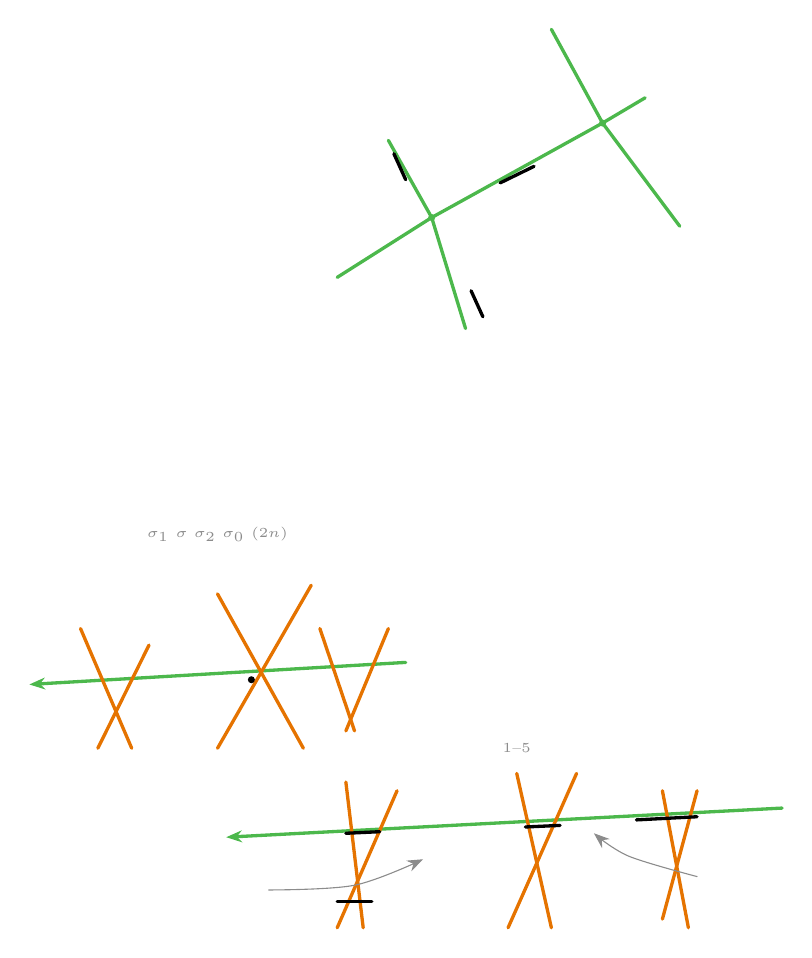
\begin{tikzpicture}[x=1mm,y=1mm,line cap=round,line join=round,font=\scriptsize]
\draw[Lg,very thick] (53.3,-26.1) -- (75,-14.1);
\draw[Lg,very thick] (53.3,-26.1) -- (41.3,-33.7);
\draw[Lg,very thick] (53.3,-26.1) -- (57.6,-40.2);
\draw[Lg,very thick] (53.3,-26.1) -- (47.8,-16.3);
\draw[Lg,very thick] (75,-14.1) -- (68.5,-2.2);
\draw[Lg,very thick] (75,-14.1) -- (84.8,-27.2);
\draw[Lg,very thick] (75,-14.1) -- (80.4,-10.9);
\node[pt,Lg] at (53.3,-26.1) {};
\node[pt,Lg] at (75,-14.1) {};
\draw[very thick] (48.5,-18) -- (50,-21.3);
\draw[very thick] (62,-21.7) -- (66.3,-19.6);
\draw[very thick] (58.3,-35.4) -- (59.8,-38.7);
\draw[Lg,very thick,-{Stealth[length=2mm]}] (50,-82.6) -- (2.2,-85.4);
\draw[Or,very thick] (8.7,-78.3) -- (15.2,-93.5);
\draw[Or,very thick] (17.4,-80.4) -- (10.9,-93.5);
\draw[Or,very thick] (26.1,-73.9) -- (37,-93.5);
\draw[Or,very thick] (38,-72.8) -- (26.1,-93.5);
\node[pt] at (30.4,-84.8) {};
\draw[Or,very thick] (39.1,-78.3) -- (43.5,-91.3);
\draw[Or,very thick] (47.8,-78.3) -- (42.4,-91.3);
\node[inner sep=1pt,pencil] at (26.1,-66.3) {\tiny $\sigma_1\ \sigma\ \sigma_2\ \sigma_0$ ($2n$)};
\draw[Lg,very thick,-{Stealth[length=2mm]}] (97.8,-101.1) -- (27.2,-104.8);
\draw[Or,very thick] (42.4,-97.8) -- (44.6,-116.3);
\draw[Or,very thick] (48.9,-98.9) -- (41.3,-116.3);
\draw[Or,very thick] (64.1,-96.7) -- (68.5,-116.3);
\draw[Or,very thick] (71.7,-96.7) -- (63,-116.3);
\draw[Or,very thick] (82.6,-98.9) -- (85.9,-116.3);
\draw[Or,very thick] (87,-98.9) -- (82.6,-115.2);
\draw[very thick] (42.4,-104.3) -- (46.7,-104.1);
\draw[very thick] (65.2,-103.5) -- (69.6,-103.3);
\draw[very thick] (79.3,-102.6) -- (87,-102.2);
\draw[very thick] (41.3,-113) -- (45.7,-113);
\draw[pencil,-{Stealth[length=2mm]}] plot[smooth, tension=0.55] coordinates {(32.6,-111.5) (43.5,-110.9) (52.2,-107.6)};
\draw[pencil,-{Stealth[length=2mm]}] plot[smooth, tension=0.55] coordinates {(87,-109.8) (78.3,-107.2) (73.9,-104.3)};
\node[inner sep=1pt,pencil] at (64.1,-93.5) {\tiny $1$--$5$};
\end{tikzpicture}
\end{document}
